\documentclass[11pt]{article}

\usepackage{fullpage}
\usepackage{newtxtext}
\usepackage{microtype}
\usepackage[T1]{fontenc}

\usepackage{hyperref}
\hypersetup{hypertexnames=false,breaklinks=true,colorlinks=true,linkcolor=blue,filecolor=blue,citecolor=blue,urlcolor=blue}

\usepackage{mathtools}
% show equation numbers only for referenced equations
\mathtoolsset{showonlyrefs}

\usepackage{amsfonts,amssymb}
\usepackage[amsmath,amsthm,thmmarks,hyperref]{ntheorem}
\usepackage{thmtools}

\usepackage{enumitem}

\usepackage{zref-clever}
\zcsetup{
        cap=true, % capitalize types
        nameinlink,
}
% for migration from cleveref
\newcommand{\cref}[1]{\zcref{#1}}
\newcommand{\Cref}[1]{\zcref[S]{#1}}

%%% BLACKBOARD SYMBOLS

\newcommand{\C}{\ensuremath{\mathbb{C}}}
\newcommand{\D}{\ensuremath{\mathbb{D}}}
\newcommand{\F}{\ensuremath{\mathbb{F}}}
\newcommand{\G}{\ensuremath{\mathbb{G}}}
\newcommand{\J}{\ensuremath{\mathbb{J}}}
\newcommand{\N}{\ensuremath{\mathbb{N}}}
\newcommand{\Q}{\ensuremath{\mathbb{Q}}}
\newcommand{\R}{\ensuremath{\mathbb{R}}}
\newcommand{\T}{\ensuremath{\mathbb{T}}}
\newcommand{\Z}{\ensuremath{\mathbb{Z}}}
\newcommand{\QR}{\ensuremath{\mathbb{QR}}}

\newcommand{\Zt}{\ensuremath{\Z_t}}
\newcommand{\Zp}{\ensuremath{\Z_p}}
\newcommand{\Zq}{\ensuremath{\Z_q}}
\newcommand{\ZN}{\ensuremath{\Z_N}}
\newcommand{\Zps}{\ensuremath{\Z_p^*}}
\newcommand{\ZNs}{\ensuremath{\Z_N^*}}
\newcommand{\JN}{\ensuremath{\J_N}}
\newcommand{\QRN}{\ensuremath{\QR_{N}}}
\newcommand{\QRp}{\ensuremath{\QR_{p}}}

%%% THEOREM COMMANDS

\declaretheorem[numberwithin=section]{theorem}

\declaretheorem[sibling=theorem,style=plain]
        {lemma,corollary,proposition,claim,fact}

\declaretheorem[sibling=theorem,style=definition]
        {definition,conjecture,construction,assumption,protocol}

\declaretheorem[sibling=theorem,style=remark]
        {remark,example,note}

% teach zref-clever these names

\zcRefTypeSetup{claim}{Name-sg=Claim,Name-pl=Claims,name-sg=claim,name-pl=claims}
\zcRefTypeSetup{fact}{Name-sg=Fact,Name-pl=Facts,name-sg=fact,name-pl=facts}
\zcRefTypeSetup{maintheorem}{Name-sg=Main Theorem,Name-pl=Main
Theorems,name-sg=main theorem,name-pl=main theorems}
\zcRefTypeSetup{conjecture}{Name-sg=Conjecture,Name-pl=Conjectures,name-sg=conjecture,name-pl=conjectures}
\zcRefTypeSetup{construction}{Name-sg=Construction,Name-pl=Constructions,name-sg=construction,name-pl=constructions}
\zcRefTypeSetup{assumption}{Name-sg=Assumption,Name-pl=Assumptions,name-sg=assumption,name-pl=assumptions}
\zcRefTypeSetup{protocol}{Name-sg=Protocol,Name-pl=Protocols,name-sg=protocol,name-pl=protocols}
\zcRefTypeSetup{question}{Name-sg=Question,Name-pl=Questions,name-sg=question,name-pl=questions}

% equation numbering style
\numberwithin{equation}{section}

%%% GENERAL COMPUTING

\newcommand{\bit}{\ensuremath{\set{0,1}}}
\newcommand{\pmone}{\ensuremath{\set{-1,1}}}

% asymptotics
\DeclareMathOperator{\poly}{poly}
\DeclareMathOperator{\polylog}{polylog}
\DeclareMathOperator{\negl}{negl}
\newcommand{\Otil}{\ensuremath{\tilde{O}}}

% probability/distribution stuff
\DeclareMathOperator*{\E}{E}
\DeclareMathOperator*{\Var}{Var}

% sets in calligraphic type
\newcommand{\calD}{\ensuremath{\mathcal{D}}}
\newcommand{\calF}{\ensuremath{\mathcal{F}}}
\newcommand{\calG}{\ensuremath{\mathcal{G}}}
\newcommand{\calH}{\ensuremath{\mathcal{H}}}
\newcommand{\calX}{\ensuremath{\mathcal{X}}}
\newcommand{\calY}{\ensuremath{\mathcal{Y}}}

% types of indistinguishability
\newcommand{\compind}{\ensuremath{\stackrel{c}{\approx}}}
\newcommand{\statind}{\ensuremath{\stackrel{s}{\approx}}}
\newcommand{\perfind}{\ensuremath{\equiv}}

% font for general-purpose algorithms
\newcommand{\algo}[1]{\ensuremath{\mathsf{#1}}}
% font for general-purpose computational problems
\newcommand{\problem}[1]{\ensuremath{\mathsf{#1}}}
% font for complexity classes
\newcommand{\class}[1]{\ensuremath{\mathsf{#1}}}

% complexity classes and languages
\renewcommand{\P}{\class{P}}
\newcommand{\BPP}{\class{BPP}}
\newcommand{\NP}{\class{NP}}
\newcommand{\coNP}{\class{coNP}}
\newcommand{\AM}{\class{AM}}
\newcommand{\coAM}{\class{coAM}}
\newcommand{\IP}{\class{IP}}

%%% "LEFT-RIGHT" PAIRS OF SYMBOLS


% inner product
\DeclarePairedDelimiter\inner{\langle}{\rangle}
% absolute value
\DeclarePairedDelimiter\abs{\lvert}{\rvert}
% a set
\DeclarePairedDelimiter\set{\{}{\}}
% parens
\DeclarePairedDelimiter\parens{(}{)}
% tuple, alias for parens
\DeclarePairedDelimiter\tuple{(}{)}
% square brackets
\DeclarePairedDelimiter\bracks{[}{]}
% rounding off
\DeclarePairedDelimiter\round{\lfloor}{\rceil}
% floor function
\DeclarePairedDelimiter\floor{\lfloor}{\rfloor}
% ceiling function
\DeclarePairedDelimiter\ceil{\lceil}{\rceil}
% length of some vector, element
\DeclarePairedDelimiter\length{\lVert}{\rVert}
% "lifting" of a residue class
\DeclarePairedDelimiter\lift{\llbracket}{\rrbracket}
\DeclarePairedDelimiter\len{\lvert}{\rvert}

%%% CRYPTO-RELATED NOTATION

% KEYS AND RELATED

\newcommand{\key}[1]{\ensuremath{#1}}

\newcommand{\pk}{\key{pk}}
\newcommand{\vk}{\key{vk}}
\newcommand{\sk}{\key{sk}}
\newcommand{\mpk}{\key{mpk}}
\newcommand{\msk}{\key{msk}}
\newcommand{\fk}{\key{fk}}
\newcommand{\id}{id}
\newcommand{\keyspace}{\ensuremath{\mathcal{K}}}
\newcommand{\msgspace}{\ensuremath{\mathcal{M}}}
\newcommand{\ctspace}{\ensuremath{\mathcal{C}}}
\newcommand{\tagspace}{\ensuremath{\mathcal{T}}}
\newcommand{\idspace}{\ensuremath{\mathcal{ID}}}

\newcommand{\concat}{\ensuremath{\|}}

% GAMES

% advantage
\newcommand{\advan}{\ensuremath{\mathbf{Adv}}}

% different attack models
\newcommand{\attack}[1]{\ensuremath{\text{#1}}}

\newcommand{\atk}{\attack{atk}} % dummy attack
\newcommand{\indcpa}{\attack{ind-cpa}}
\newcommand{\indcca}{\attack{ind-cca}}
\newcommand{\anocpa}{\attack{ano-cpa}} % anonymous
\newcommand{\anocca}{\attack{ano-cca}}
\newcommand{\euacma}{\attack{eu-acma}} % forgery: adaptive chosen-message
\newcommand{\euscma}{\attack{eu-scma}} % forgery: static chosen-message
\newcommand{\suacma}{\attack{su-acma}} % strongly unforgeable

% ADVERSARIES
\newcommand{\attacker}[1]{\ensuremath{\mathcal{#1}}}

\newcommand{\Adv}{\attacker{A}}
\newcommand{\AdvA}{\attacker{A}}
\newcommand{\AdvB}{\attacker{B}}
\newcommand{\Dist}{\attacker{D}}
\newcommand{\Sim}{\attacker{S}}
\newcommand{\Ora}{\attacker{O}}
\newcommand{\Inv}{\attacker{I}}
\newcommand{\For}{\attacker{F}}

% CRYPTO SCHEMES

\newcommand{\scheme}[1]{\ensuremath{\text{#1}}}

% pseudorandom stuff
\newcommand{\prg}{\algo{PRG}}
\newcommand{\prf}{\algo{PRF}}
\newcommand{\prp}{\algo{PRP}}

% symmetric-key cryptosystem
\newcommand{\skc}{\scheme{SKC}}
\newcommand{\skcgen}{\algo{Gen}}
\newcommand{\skcenc}{\algo{Enc}}
\newcommand{\skcdec}{\algo{Dec}}

% public-key cryptosystem
\newcommand{\pkc}{\scheme{PKC}}
\newcommand{\pkcgen}{\algo{Gen}}
\newcommand{\pkcenc}{\algo{Enc}} % can also use \kemenc and \kemdec
\newcommand{\pkcdec}{\algo{Dec}}

% digital signatures
\newcommand{\sig}{\scheme{SIG}}
\newcommand{\siggen}{\algo{Gen}}
\newcommand{\sigsign}{\algo{Sign}}
\newcommand{\sigver}{\algo{Ver}}

% message authentication code
\newcommand{\mac}{\scheme{MAC}}
\newcommand{\macgen}{\algo{Gen}}
\newcommand{\mactag}{\algo{Tag}}
\newcommand{\macver}{\algo{Ver}}

% key-encapsulation mechanism
\newcommand{\kem}{\scheme{KEM}}
\newcommand{\kemgen}{\algo{Gen}}
\newcommand{\kemenc}{\algo{Encaps}}
\newcommand{\kemdec}{\algo{Decaps}}

% identity-based encryption
\newcommand{\ibe}{\scheme{IBE}}
\newcommand{\ibesetup}{\algo{Setup}}
\newcommand{\ibeext}{\algo{Ext}}
\newcommand{\ibeenc}{\algo{Enc}}
\newcommand{\ibedec}{\algo{Dec}}

% hierarchical IBE (as key encapsulation)
\newcommand{\hibe}{\scheme{HIBE}}
\newcommand{\hibesetup}{\algo{Setup}}
\newcommand{\hibeext}{\algo{Extract}}
\newcommand{\hibeenc}{\algo{Encaps}}
\newcommand{\hibedec}{\algo{Decaps}}

% binary tree encryption (as key encapsulation)
\newcommand{\bte}{\scheme{BTE}}
\newcommand{\btesetup}{\algo{Setup}}
\newcommand{\bteext}{\algo{Extract}}
\newcommand{\bteenc}{\algo{Encaps}}
\newcommand{\btedec}{\algo{Decaps}}

% trapdoor functions
\newcommand{\tdf}{\scheme{TDF}}
\newcommand{\tdfgen}{\algo{Gen}}
\newcommand{\tdfeval}{\algo{Eval}}
\newcommand{\tdfinv}{\algo{Invert}}
\newcommand{\tdfver}{\algo{Ver}}

%%% PROTOCOLS

\newcommand{\out}{\text{out}}
\newcommand{\view}{\text{view}}

%%% COMMANDS FOR LECTURES/HOMEWORKS

\RequirePackage{fancyhdr}

\newcommand{\lecheader}{%
  \chead{\large \textbf{Lecture \lecturenum\\\lecturetopic}}

  \lhead{\small
    \textbf{\href{https://github.com/cpeikert/TheoryOfCryptography}{Theory
        of Cryptography}}\\}

  \rhead{\small \textbf{Instructor:
      \href{http://www.eecs.umich.edu/~cpeikert/}{Chris Peikert}\\Scribe:
      \scribename}}

  \setlength{\headheight}{20pt}
  \setlength{\headsep}{16pt}
}


%%% xsim settings

\RequirePackage{xsim}
\RequirePackage{needspace}

\DeclareExerciseEnvironmentTemplate{QRef}{%
    \par\addvspace{\baselineskip}
    \Needspace*{2\baselineskip}
    \noindent
    \hyperref[ans:\GetExerciseProperty{ID}]{\textbf{\XSIMmixedcase{\GetExerciseName}~\GetExerciseProperty{counter}.}}
    \label{ques:\GetExerciseProperty{ID}}
}{\par\addvspace{\baselineskip}}

\DeclareExerciseEnvironmentTemplate{ARef}{%
        \Needspace*{2\baselineskip}
        \noindent
        \hyperref[ques:\GetExerciseProperty{ID}]{\textbf{\XSIMmixedcase{\GetExerciseParameter{exercise-name}}~\GetExerciseProperty{counter}.}}
        \label{ans:\GetExerciseProperty{ID}}
        \GetExerciseBody{exercise}
        \par \medskip \noindent
        \textbf{\XSIMmixedcase{\GetExerciseName}.}
}{\par\addvspace{\baselineskip}}

\DeclareExerciseHeadingTemplate{simple}{%
    \section*{\XSIMmixedcase{\GetExerciseParameter{solution-name}s}}
}

\DeclareExerciseType{question}{%
    exercise-env = question,
    solution-env = answer,
    exercise-name = Question,
    solution-name = Answer,
    exercise-template = QRef,
    solution-template = ARef,
}

\xsimsetup{%
  path = {questions},
  file-extension = {aux},
  print-solutions/headings-template=simple,
  exercise/template=runin
}

\loadxsimstyle{layouts}

\AtEndDocument{\pagebreak\printsolutions}


\usepackage{algorithm,algorithmic}
\usepackage{tikz}
\usetikzlibrary{arrows.meta,decorations.pathreplacing,fit,positioning}

% VARIABLES

\newcommand{\lecturenum}{6}
\newcommand{\lecturetopic}{Pseudorandom Generators, Blum-Micali}
\newcommand{\scribename}{Alessio Guerrieri}

% END OF VARIABLES

\lecheader

\pagestyle{plain}               % default: no special header

\begin{document}

\thispagestyle{fancy}           % first page should have special header

% LECTURE MATERIAL STARTS HERE

\section{Pseudorandom Generators}
\label{sec:prgs}

The pioneering computer scientist John von Neumann said, “Anyone who considers arithmetical methods of producing random digits is, of course, in a state of sin.”
By this he meant that deterministic procedures cannot generate randomness from nothing: their outputs are completely determined by their inputs.
More generally, a deterministic procedure cannot increase randomness in an information-theoretic sense (see the question below).

A \emph{pseudorandom generator} sidesteps this limitation: it is an efficient deterministic procedure that transforms a random input into a longer string that \emph{appears} uniformly random to any efficient procedure, in the sense of computational indistinguishability.
It is formalized as follows.

\begin{definition}
  \label{def:prg}
  A \emph{deterministic} function $G : \bit^{*} \to \bit^{*}$ is a \emph{pseudorandom generator} (PRG) with \emph{expansion} $\ell(n) > n$ if:
  \begin{itemize}
  \item $G$ can be evaluated by a polynomial-time algorithm,
  \item $\len{G(x)} = \ell(\len{x}) > \len{x}$ for all $x \in \bit^{*}$ (or more generally, whose length is an allowed security parameter), and
  \item the ensemble $\set{G(U_{n})}$ is pseudorandom, i.e., $\set{G(U_{n})} \compind \set{U_{\ell(n)}}$.
  \end{itemize}
\end{definition}

The final property is very strong: by the composition lemma, it follows that $G(U_{n})$ can be used in place of $U_{\ell(n)}$ in \emph{any} efficient algorithm, with computationally indistinguishable results.

For any PRG~$G$ with expansion $\ell(n)$, the image $G(\bit^n)$ contains at most $2^n$ strings, a fraction at most $1/2^{\ell(n)-n}$ of all $\ell(n)$-bit strings.
When, e.g., $\ell(n)\geq 2n$, this fraction is exponentially small, yet no PPT algorithm can distinguish (with non-negligible advantage) the output of~$G$ on a uniform seed from a uniformly random string.

\begin{question}
  Prove (or at least sketch a proof) that a \emph{statistically} pseudorandom generator cannot exist.
  \emph{Hint:} think about the sizes of $G(\bit^n)$ and $\bit^{\ell(n)}$, and define an appropriate statistical test (i.e., subset of $\bit^{\ell(n)}$).
\end{question}

\begin{answer}
  Since $G$ has $n$-bit seeds (of which there are $2^n$), there are at most $2^n$ possible outputs of $G$ (which reside in $\bit^{\ell(n)}$).
  However, $\bit^{\ell(n)}$ is significantly larger than this; it has $2^{\ell(n)} \geq 2^{n+1}$ elements, making it at least twice as big as the image of \(G\).
  Informally, we can think of our statistical test as checking whether or not its given string is in the image of $G$.
  When the string is an output of~$G$, the check always succeeds; when the string is uniformly random, there is a significant (at least $1/2$) probability that the check fails.

  More formally and in the language of statistical indistinguishably: let $A = G(\bit^n) \subseteq \bit^{\ell(n)}$, i.e., the image of $G$, as suggested above.
  Because~$G$ is deterministic, we have $\abs{A} \leq 2^{n}$.
  Then
  \[
    \begin{aligned}
      \abs{G(U_n)(A) - U_{\ell(n)}(A)}
      &= \abs{1 - U_{\ell(n)}(A)} \\
      &= 1 - \abs{A} \cdot 2^{-\ell(n)}  \\
      &\geq 1 - 2^{n-\ell(n)} \\
      &\geq 1 - 2^{-1} = 1/2,
    \end{aligned}
  \]
  which is non-negligible.
  Since we have demonstrated a particular~$A$ for which $\abs{G(U_n)(A) - U_{\ell(n)}(A)} \geq 1/2$, the suprenum over all possible~$A$ cannot be smaller, so $\Delta(G(U_n), U_{\ell(n)}) \geq 1/2$.
\end{answer}

\section{Expanding a PRG}
\label{sec:expanding-prg}

The smallest possible PRG expansion is one bit: $\ell(n)=n+1$.
It turns out that this is sufficient to obtain \emph{any} polynomial expansion!

\begin{theorem}
  \label{thm:prg-expansion}
  Suppose that there exists a PRG~$G$ with expansion $\ell(n)=n+1$.
  Then for any integer-valued $t(n)>n$ such that $1^{t(n)}$ is polynomial-time computable from $1^n$ (hence $t(n)=\poly(n)$), there exists a PRG~$G_t$ with expansion $t(n)$.
\end{theorem}

\begin{proof}
  We will construct $G_t(s)$ from $G$.
  Our construction applies~$G$ $t(n)$ times, outputting one new bit at each step and using the other~$n$ bits of the previous step's output as the next seed; see the following picture.

  \begin{figure}[h!]
    \centering
    \begin{tikzpicture}[
      >={Stealth[length=1.5mm]},
      generator/.style={draw, minimum width=8mm, minimum height=11mm},
      wire/.style={->, semithick},
      bit count/.style={midway, above, font=\small},
      every node/.style={inner sep=2pt}
    ]
      \node[generator] (g1) {$G$};
      \node[generator, right=15mm of g1] (g2) {$G$};
      \node[generator, right=15mm of g2] (g3) {$G$};
      \node[right=8mm of g3] (dots) {$\cdots$};
      \node[generator, right=8mm of dots] (gt) {$G$};
      \node[left=12mm of g1] (seed) {$s$};
      \node[right=15mm of gt, font=\small] (discard) {discard};

      \draw[wire] (seed) -- node[bit count] {$n$ bits} (g1);
      \draw[wire] (g1) -- node[bit count] {$n$ bits} (g2);
      \draw[wire] (g2) -- node[bit count] {$n$ bits} (g3);
      \draw[wire] (g3) -- (dots);
      \draw[wire] (dots) -- (gt);
      \draw[wire] (gt) -- node[bit count] {$n$ bits} (discard);

      \node[below=10mm of g1] (b1) {$b_1$};
      \node[below=10mm of g2] (b2) {$b_2$};
      \node[below=10mm of g3] (b3) {$b_3$};
      \node[below=10mm of gt] (bt) {$b_{t(n)}$};
      \node at (dots |- b1) {$\cdots$};
      \foreach \g/\b in {g1/b1,g2/b2,g3/b3,gt/bt}
        \draw[wire] (\g.south) -- node[midway, right, font=\small] {1 bit} (\b.north);
      \node[fit=(b1)(b2)(b3)(bt), inner sep=2pt] (output) {};
      \draw[decorate, decoration={brace, mirror, amplitude=4pt}]
        (output.south west) -- node[below=6pt, font=\small] {output} (output.south east);
    \end{tikzpicture}
  \end{figure}

  Formally, for any nonnegative integer~$k$, let $G_k(s)$ denote the procedure from \cref{alg:Gk}, which produces~$k$ output bits from an $n$-bit seed~$s$.
  \begin{algorithm}[h]
    \caption{$G_k(s)$}
    \begin{algorithmic}
      \IF{$k = 0$} \RETURN $\varepsilon$ (the empty string)
      \ELSE \STATE let $(x|b)=G(s)$, where $x \in \bit^{n}$, $b \in \bit$
      \RETURN $b|G_{k-1}(x)$
      \ENDIF
    \end{algorithmic}
    \label{alg:Gk}
  \end{algorithm}
  The desired generator uses $k=t(n)$ on seeds of length~$n$; we abbreviate $G_{t(n)}(s)$ as $G_t(s)$.
  By construction, its output has length $t(n)$.
  Since $t(n)$ is efficiently computable and polynomially bounded, and~$G$ is polynomial-time and called only on inputs of length~$n$, $G_{T}$ runs in polynomial time.

  It remains to prove that $\set{G_t(U_n)}\compind\set{U_{t(n)}}$.
  Each invocation of~$G$ produces both an output bit and the seed for the next invocation, so these may be correlated.
  We must establish pseudorandomness of the entire output, accounting for these correlations.
  To prove this, we define a sequence of \emph{hybrid} distributions going from the ``real'' output distribution $G_t(U_n)$ to the ``ideal'' uniform distribution $U_{t(n)}$.
  We then give a single algorithm that, given the index of an adjacent pair of hybrids, maps $G(U_n)$ to the earlier one and $U_{n+1}$ to the later one.
  This algorithm will satisfy the conditions of the ``polynomially many hybrid steps'' corollary in Lecture~5, which combines the composition and hybrid lemmas to conclude that the first and last hybrid ensembles are computationally indistinguishable.

  To give some intuition about how we design the hybrid experiments, we imagine that instead of invoking the first $G$ on $n$ uniform bits, what if we replaced its output with $n+1$ truly uniform bits?
  Intuitively, these two cases should not be distinguishable, because $G$ is a PRG.
  And then what if we similarly replaced the first two invocations of $G$, and so on?
  Eventually, we would end up with $t = t(n)$ truly uniform output bits, as desired.
  Formally, the hybrid experiments are defined as follows:
  \begin{itemize}[itemsep=0pt]
  \item $H_0 = G_t(U_n)$,
  \item $H_1 = U_1 | G_{t-1}(U_n)$,
  \item In general, $H_i = U_i | G_{t-i}(U_n)$ for $i \in \set{0} \cup [t]$,
  \item so $H_t = U_{t}$.
  \end{itemize}
  (Here $t=t(n)$, and we suppress the dependence of the hybrids on~$n$.)
  All uniform strings in these expressions are sampled independently.

  Define the algorithm $\Sim(1^n,i,z)$ below, and write $\Sim_i(1^n,z):=\Sim(1^n,i,z)$.
  \begin{algorithm}[h]
    \caption{$\Sim(1^n,i,z)$ for $i\in[t(n)]$ and $z\in\bit^{n+1}$}
    \begin{algorithmic}
      \STATE parse $z$ as $(x|b)$ for $x \in \bit^{n}$, $b \in \bit$
      \RETURN $U_{i-1} | b | G_{t-i}(x)$
    \end{algorithmic}
  \end{algorithm}

  This algorithm runs in polynomial time uniformly over $i\in[t(n)]$, because it samples at most $t(n)$ bits and makes at most $t(n)$ calls to~$G$.
  If the input comes from $G(U_n)$, the recursive definition of~$G_k$ gives
  \[
    \Sim_i(1^n,G(U_n))\equiv U_{i-1}\concat G_{t-i+1}(U_n)\equiv H_{i-1}\text.
  \]
  If the input comes from $U_{n+1}$, then~$x$ and~$b$ are independent and uniform, so
  \[
    \Sim_i(1^n,U_{n+1})\equiv U_{i-1}\concat U_1\concat G_{t-i}(U_n) \equiv U_i\concat G_{t-i}(U_n)\equiv H_i\text.
  \]
  These equivalences hold for every $i\in[t(n)]$.
  Since~$G$ is a PRG, the poly-many-hybrids corollary from Lecture~5 applies with $m(n)=t(n)$, $X_n=G(U_n)$, and $Y_n=U_{n+1}$, giving $\set{G_t(U_n)}\compind\set{U_{t(n)}}$, as required.
\end{proof}

\noindent To recap, our proof of \cref{thm:prg-expansion} took the following path:
\begin{itemize}
\item We defined a construction: the candidate PRG $G_t$.
\item We defined a sequence of hybrid experiments.
  In each step, we successively replaced \emph{one} ``real'' invocation of a crypto primitive ($G(U_{n})$) with its ``ideal'' counterpart ($U_{n+1}$).
\item We gave a single algorithm~$\Sim$ taking a hybrid index~$i$ as input, and verified that it maps $G(U_n)$ to the $(i-1)$st hybrid and $U_{n+1}$ to the $i$th hybrid.
\item This~$\Sim$ is PPT, and $\set{G(U_{n})} \compind \set{U_{n+1}}$ by hypothesis, so the polynomial-step corollary implies that the initial and final hybrid ensembles are computationally indistinguishable.
\end{itemize}

\section{Obtaining a PRG}
\label{sec:obtaining-prg}

Thanks to \cref{thm:prg-expansion}, we know that all we need is to obtain a PRG with one extra bit of output.
We describe a number-theoretic construction, due to Blum and Micali, of such an object.

\subsection{Number Theory Background}
\label{sec:background}

\begin{theorem}[Euler's theorem]
  \label{thm:euler-thm}
  Let $G$ be a finite abelian (i.e., commutative) multiplicative group.
  For every $a \in G$, we have $a^{\abs{G}} = 1$.
\end{theorem}

\begin{proof}
  Consider the set $A = a \cdot G = \set{ ax\; :\; x \in G}$.
  Because $G$ is a group, $a$ is invertible, and we have $A = G$.
  Taking products over all elements in $A = G$, we have \[ \prod_{x \in G} (ax) = \prod_{x \in G} x.
  \] Because $G$ is commutative, the LHS is $a^{\abs{G}} \cdot \prod_{x \in G} x$, and we can multiply by the inverse of the RHS to obtain $a^{\abs{G}} = 1$.
\end{proof}

When $G = \Zp^{*}$ for a prime $p$, we have $\abs{\Zp^{*}} = \varphi(p) = p-1$, so we obtain the following corollary:

\begin{corollary}[Fermat's ``little'' theorem]
  Let $p$ be a prime.
  For any $a \in \Zp^{*}$, we have $a^{p-1} = 1 \bmod p$.
\end{corollary}

The following structural theorem will be very useful.
(Its proof is elementary bur rather tedious, so we won't go through it today.)

\begin{theorem}
  \label{thm:Zps-cyclic}
  Let $p$ be a prime.
  The multiplicative group $\Zp^{*}$ is \emph{cyclic}, i.e., there exists some \emph{generator} $g \in \Zp^{*}$ such that $\Zp^{*} = \langle g \rangle := \set{g^{1}, g^{2}, \ldots, g^{p-1}=g^{0}=1}$.
  (Equivalently, we can write the group as $\Zp^{*} = \set{g^{0}, g^{1}, \ldots, g^{p-2}}$.)
\end{theorem}

\begin{question}
  Suppose there is a ``black box'' \(\algo{B}\) that outputs a uniformly random element of \(\Z_{p-1}\) for some known prime \(p\).
  Show that there exists an algorithm that, using~\(\algo{B}\) as its only source of randomness, samples a uniformly random element of \(\Z_p^*\).
\end{question}

\begin{answer}
  By \cref{thm:Zps-cyclic}, there exists a generator~\(g\) of~\(\Zp^{*}\).
  So, there exists an algorithm \(\algo{A}\) that simply samples an $x \gets \algo{B}$ and returns \(g^{x}\).
  By \cref{thm:Zps-cyclic}, we know that \(\inner{g} = \set{g^0, \ldots, g^{p-2}} = \Z_p^*\), and since \(\abs{\Z_p^*} = p - 1\), it must be the case that for each \(x \in \Z_p^*\), there exists a \emph{unique} \(i \in \Z_{p-1}\) such that \(x = g^i\).
  Hence, \(\Pr[\algo{A} \text{ outputs } x] = \Pr[B \text{ outputs } i] = 1/(p-1)\), as needed.
\end{answer}

\subsection{Discrete Logarithm Problem and One-Way Function}
\label{sec:dlp-owf}

\Cref{thm:Zps-cyclic} leads naturally to the so-called \emph{discrete logarithm problem}, which is: given $y \in \Zp^{*}$ (and prime $p$ and generator $g$ of $\Zp^{*}$), find $\log_{g} y$, i.e., the $x \in \set{1, \ldots, p-1}$ for which $y = g^{x} \bmod p$.
This problem is believed to be infeasible for large values of $p$.

\begin{conjecture}[Discrete logarithm assumption]
  Let $\algo{S}(1^{n})$ be a PPT algorithm that outputs some prime $p$ and generator $g$ of $\Zp^{*}$.
  For every PPT algorithm $\Adv$, \[ \Pr_{(p,g) \gets \algo{S}(1^{n}), y \gets \Zp^{*}} [\Adv(p,g,y) = \log_{g} y] = \negl(n).
\]
\end{conjecture}

We would like to design a collection of OWFs based on the discrete logarithm assumption.
The collection is made up of the functions $f_{p,g} \colon \set{1, \ldots, p-1} \to \Zp^{*}$ (for prime $p$ and generator $g$ of $\Zp^{*}$), defined as
\[ f_{p,g}(x) = g^{x} \bmod p. \] Moreover, these functions are even
\emph{permutations} if we identify $\set{1, \ldots, p-1}$ with
$\Zp^{*}$ in the natural way.

It is a tautology that the collection is one-way under the discrete logarithm assumption.
It is also clear that we can efficiently sample from the domain of $f_{p,g}$.
But we still need to check that $f_{g,p}$ can be evaluated efficiently, and that $(p,g)$ can be generated efficiently.

For the first, we use the standard ``repeated squaring'' technique for exponentiation, which requires $O(\len{x})$ multiplications modulo $p$.
The solution to the second issue is not entirely straightforward.
Given only the prime $p$, it is unknown (in general) how to find a generator $g$ of $\Zp^{*}$ efficiently.
However, given the \emph{factorization} of $p-1$, which can be generated along with $p$, it is possible: every element in $\Zp^{*}$ has order dividing $p-1$, so $g$ is a generator if and only if $g^{(p-1)/q} \neq 1 \bmod p$ for every prime divisor $q$ of $p-1$.
The number of non-generators is at most the sum of $(p-1)/q$ over all prime divisors $q$ of $p-1$, so the density of generators is typically large enough.
An often-used special case is $p = 2q+1$ for prime $q$, for which there are $q = (p-1)/2$ generators.
However, it is not even known whether there exist infinitely many such ``Sophie Germain'' primes of this form!
(Empirically, though, they are abundant.)

%% TODO: think of a question for the end of this section

\subsection{Blum-Micali PRG}
\label{sec:blum-micali-prg}

We now present a PRG that uses the ideas presented in the previous section.
From \cref{sec:expanding-prg} we know that if we have a PRG that is able to generate one extra bit of randomness, we can generate a polynomial number of pseudorandom bits.
Our goal will be the following: we want to construct a PRG $G_{p,g} \colon \Zp^* \to \Zp^* \times \bit$.\footnote{To be pedantic, $G_{p,g}$ is a ``collection'' of PRGs, where the input seed comes from a set that depends on the function index $(p,g)$.
  It it easy to check that our construction from \cref{sec:expanding-prg} is compatible with this collection $G_{p,g}$.}

Our solution is a function with the following form: \[ G_{p,g}(x)= (f_{p,g}(x)=g^x \bmod p \quad, \quad h(x)).
\] Note that $f_{p,g}(x)$ performs the modular exponentiation function (which is a one-way under the discrete log assumption), while $h \colon \Zp^{*} \to \bit$ is some function (yet to be defined) that provides the additional bit.

Looking at the function, we can make the following observation: if $x \in \Zp^{*}$ is chosen uniformly at random, then also $f_{p,g}(x)$ is uniform (because $f_{p,g}$ is a permutation).
We still need to choose the function $h$, keeping in mind what we want from from the function: $h(x)$ should ``look like a random bit,'' \emph{even given $f_{p,g}(x)$}.
That is, $h(x)$ should compute ``something about $x$'' that $f$ hides \emph{completely}.

We can think of many possible candidates for $h$: apply the xor function to all the bit of $x$; take the least significant bit of $x$ (though you will show that this \emph{does not} meet our requirements!); take the ``most significant bit'' of $x$ (more precisely, test if $x>\frac{p-1}{2}$); etc.

Let's formalize the security property we want from~$h$.
Informally, we want it to be the case that no efficient algorithm, given $f(x)$, should be able to guess $h(x)$ with probability much better than the~$\frac{1}{2}$ that is achievable by random guessing.

\begin{definition}[Hard-core predicate]
  \label{def:hard-core-pred}
  A predicate $h \colon \bit^* \to \bit$ is \emph{hard-core} for~$f$ if for all PPT algorithms $\Adv$,
  \[ \advan_{f,h}(\Adv) := \Pr_{x}[\Adv(f(x))=h(x)] - \frac12 = \negl(n).
  \]
\end{definition}

Next time, we will show that under the discrete log assumption, the ``most significant bit'' predicate $h(x) = [x > \frac{p-1}{2}]$ is hard-core for $f_{p,g}$.

\begin{question}
  Prove that if $h$ is hard-core for a one-way permutation $f \colon D \to D$, then
  \[ (f(x),h(x)) \compind (U(D),U_1) \equiv (f(x),b), \] where $x \gets D$ and $b \gets \bit$ are independent.
  This means that $G(x)=(f(x),h(x)) \in D \times \bit$ is a PRG that expands by one bit.
  \emph{Hint:} give a reduction that converts any distinguisher for the above two distributions into a predictor of~$h(x)$ given~$f(x)$.
\end{question}

\begin{answer}
  We prove this by reduction.
  Let~$\calD$ be a PPT algorithm that seeks to distinguish $(f(x),h(x))$ from $(f(x), b)$, where $x \gets D, b \gets \bit$ are independent.
  We construct a PPT predictor~$\AdvA$ against the hard-core predicate~$h$ for~$f$, which uses~$\calD$ as a black box and has the same advantage.
  The key idea is that~$\AdvA$, given some $y=f(x)$ for unknown~$x$, will simply guess a candidate value~$b$ for the hard-core bit~$h(x)$, and invoke~$\calD(y,b)$ to get some indication of whether this guess is correct.
  Since~$\calD$ may not be a perfect distinguisher, its answer may not always be ``correct,'' so it requires some care to analyze this reduction.

  Formally, we define the predictor~$\AdvA$ to work as follows: given input $y \in D$, choose a uniformly random bit $b \gets \bit$ and invoke $\calD(y,b)$.
  If~$\calD$ accepts (i.e., outputs 1), then output~$b$ as the prediction for $h(f^{-1}(y))$; otherwise, output $\overline{b}$ as the prediction.
  Clearly, $\AdvA$ is PPT.

  We now relate $\AdvA$'s advantage in the prediction game to $\calD$'s advantage in the distinguishing game.
  First, observe that $\AdvA$'s advantage is
  \begin{align*}
    \advan(\AdvA)
    &= \Pr_{x \gets D}[\AdvA(f(x))=h(x)] - 1/2 \\
    &= \frac12 \parens*{\Pr_{x \gets D}[\calD(f(x),h(x))=1] + \Pr_{x
      \gets D}[\calD(f(x),\overline{h(x)})=0] - 1} \\
    &= \frac12 \parens*{\Pr_{x \gets D}[\calD(f(x),h(x))=1] - \Pr_{x
      \gets D}[\calD(f(x),\overline{h(x)})=1]},
  \end{align*}
  because~$\AdvA(f(x))$ outputs the correct bit~$h(x)$ if~$\AdvA$ chooses $b=h(x)$ and $\calD(f(x),b)$ accepts, or if~$\AdvA$ chooses $b=\overline{h(x)}$ and $\calD(f(x),b)$ rejects.
  These events are disjoint, so we can add their probabilities, and~$b$ is uniform and independent of~$x$, leading to the $1/2$ factor.

  Now let
  \begin{align*}
    p_{U}
    &= \Pr_{x \gets D, b \gets \bit}[\calD(f(x),b) = 1] \\
    &= \frac12 \parens*{\Pr_{x \gets D}[\calD(f(x),h(x)) = 1] + 
      \Pr_{x \gets D}[\calD(f(x), \overline{h(x)}) = 1]},
  \end{align*}
  because each of $b=h(x)$ and $b=\overline{h(x)}$ occur with probability $1/2$.
  Similarly, define
  \[ p_{G} = \Pr_{x \gets D}[\calD(f(x), h(x))=1].
  \] By definition, $\calD$'s advantage is
  \begin{align*}
    \advan(\calD) = p_{G}-p_{U}
    &= \frac12 \parens*{\Pr_{x \gets D}[\calD(f(x),
      h(x))=1] - \Pr_{x \gets D}[\calD(f(x),\overline{h(x)})=1]} \\
    &= \advan(\AdvA).
  \end{align*}
  Since $\AdvA$'s advantage is negligible by the hypothesis that~$h$ is hard-core for~$f$, so is $\calD$'s advantage, as desired.
\end{answer}

\end{document}

%%% Local Variables: 
%%% mode: latex
%%% TeX-master: t
%%% End: 
